\chapter{The LHC and CMS Experiment}
\label{sec:cms}

\section{The LHC}

\section{The CMS Detector}

The CMS detector is a multi-purpose detector that operates on the LHC beamline at CERN. The LHC tunnel is a \(27\) km ring which was previously home to the LEP accelerator. Run-2 at the LHC ran from 2015 to 2018 at a centre of mass energy of \(\sqrt{s} = 13\) TeV. In that time, the CMS detector collected a total integrated luminosity of 163 \(\text{fb}^{-1}\). A schematic of the CMS detector is shown in Figure \ref{fig:CMS_Schematic}. The barrel of the detector is split into five sections: the silicon pixel and strip tracker, the electromagnetic calorimeter (ECAL), the hadronic calorimeter (HCAL), the superconducting solenoid and the muon detector. The detector is further enclosed with an endcap at either end of the barrel. These endcaps similarly contain a silicon tracker, ECAL and HCAL. They allow for a significant extension of the pseudorapidity coverage in the detector.

\begin{figure}[H]
    \centering
    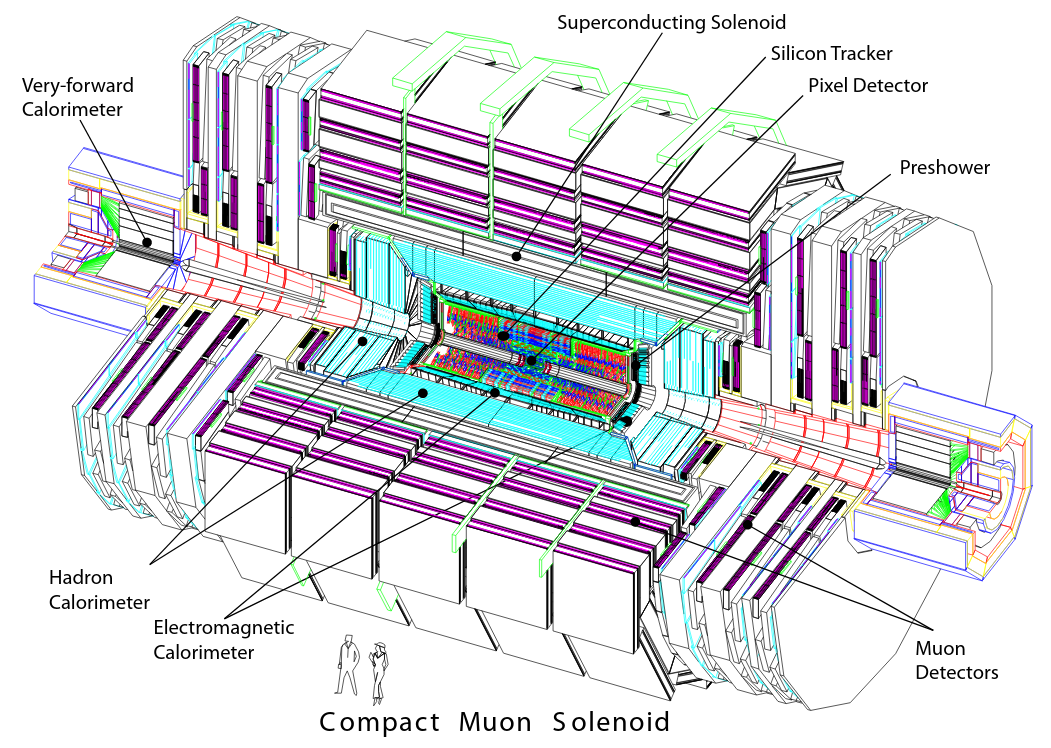
\includegraphics[scale=0.4]{Figures/CMS_Detector.png}
    \caption{A perspective view of the CMS detector \cite{CMS_Setup}.}
    \label{fig:CMS_Schematic}
\end{figure}

One of the key features of the detector is the superconducting solenoid that lies inside of the muon detector. It is a 13m long, 6m inner diameter superconducting solenoid that runs at 3.8 T and can provide a large bending power to all charged particles in the detector. Enclosed within the solenoid is the tracker, ECAL and HCAL. Placed outside of the solenoid is the muon detector. This allows for the double bend of the muon track to better identify the properties of the muon. \\

The tracker (pixel detector) subjected to the magnetic field can determine the charge to mass ratio of any charged particle that passes through. The CMS tracker is made from silicon and can measure charged particles with a pseudorapidity \(|\eta|<2.5\). In total the tracker contains 1440 silicon pixels and 15,148 silicon strip detector modules. For transverse momentum in the range \(1<p_{T}<10\) GeV and \(|\eta|<1.4\), the resolution of the track is approximately 1.5\% \cite{CMS_MSSM_Tau_2018}. The central barrel of the ECAL is made from 61,200 lead tungstate (\(\text{PbWO}_4\)) crystals and the endcaps contain 7,324 crystals each. Each crystal produces light proportional the the energy of a particle that is passing through it. Avalanche photodiodes are used as photodetectors in the barrel and vacuum phototriodes in the endcaps. This measured energy can be used in parallel with the tracker to provide an estimate for electron momenta. For a Z \(\rightarrow\) ee decay with \(p_T \approx\) 45 GeV the momentum resolution spans from 1.7\% for non showering electrons in the barrel and 4.5\% for showers in the endcaps \cite{electron_performance}. \\

The HCAL is a sampling calorimeter that uses absorbers made from brass and plastic scintillator tiles. The barrel and endcaps for the ECAL and the HCAL cover a pseudorapidity of up to \(|\eta|<3.0\). There is an additional HCAL outside of the magnetic yolk that sits around 6m away from the endcap, called the forward calorimeter. This allows a pseudorapidity coverage of \(2.9 < |\eta| < 5.0\). The muon detector is a section of the detector that lies outside the superconducting solenoid and can cover the range \(|\eta|<2.4\). The measurements taken in the muon detector use drift tubes, cathode strip chambers and resistive-plate chambers. The \(p_T\) resolution of muons, with \(20 < p_T < 100\) GeV measured in the tracker and the muon detector, ranges from 1.3\% to 2.0\% in the barrel and less than 6\% in the endcaps \cite{CMS_muon}.  \\

A two-tiered trigger system is used to select events of significance \cite{CMS_trigger}. The first tier is executed by hardware and selects events with any of a detected electron, photon, muon, tau lepton, jet, or missing transverse energy. It selects these events within 4 \(\mu\)s of the collision. The second tier of the trigger, known as the high-level trigger, is an event filter farm that has the capacity to run a version of the event reconstruction software. A complete description of the CMS detector and the triggering system can be found at Ref.\cite{CMS_Setup}.

\subsection{Tracker}
\subsection{Electromagnetic calorimeter}
\subsection{Hadron calorimeter}
\subsection{Muon system}
\subsection{Triggering}

